
\chapter{Background}
\label{ch:background}

In this chapter a fundamental background on the \ac{PGAS} paradigm is given and the relationship of \ac{PGAS} and \ac{GASPI} is explained. The basic functionality of \ac{GASPI}, \ac{OpenSHMEM} and \ac{MPI} is compared and differences between the programming models are pointed out.

\section{\acs{PGAS} Programming Model}

A common standalone computing system usually consists of one or more \acp{CPU}, local memory and an interconnection system to communicate with other systems. All components are combined on a common system board. The local memory is accessible by the \acp{CPU} of that system only. Access to the memory does not necessarily need to be symmetric over all \acp{CPU}. If the computer architecture is built in a way that memory is bound to a specific processor and latency varies depending on the processor and the requested address, the system is called a \ac{NUMA} architecture \cite[ch.~5.1]{carch}.

When programming for parallel computing systems, applications contain more than one thread of instructions. In most cases, communication has to occur between the parallel streams of instructions. The parallelism can either be implemented in terms of different threads in the same process \cite[p.~163\,ff.]{silberschatz} or by using multiple processes \cite[p.~122\,ff.]{silberschatz}. Because the address spaces of distinct processes are managed by the operating system, means of \ac{IPC} must be used to transfer data among processes. This can either be provided by the operating system directly or via additional libraries \cite[p.~130\,ff.]{silberschatz}.

To transfer data using \ac{MPI} in the most basic example, the sender process calls the function \code{MPI\_Send} while providing a pointer to a memory buffer holding the data to send along with some information about the data segment's length and its data type. The receiver calls \code{MPI\_Recv} with an appropriately sized receiving buffer. Due to the notion of separate processes, only raw data may be transferred in this way. Pointers possibly present inside the transferred data are related to the originating system and thus invalid on the receiving node or process. 

A different approach is taken by the \acf{PGAS} programming model: The general idea is to provide a distributed shared memory space as a virtual layer so that every node can access memory autonomously, \ie without the direct involvement of the remote node or process \cite[ch.~2.1.3]{diss-end}. The concept is implemented in various ways as extensions to existing programming languages such as \ac{UPC} and \ac{CAF} or as software libraries like \ac{OpenSHMEM} and \ac{GASPI} \cite[p.~9]{diss-end}. The \ac{PGAS} model has no strict definition. It is especially not defined, how the data is transferred or accessed. The examples of \ac{PGAS} implementations listed vary greatly in this aspect.  

\section{\acl{UPC}}

As a first example for a \ac{PGAS} programming language \ac{UPC} is presented. \Ac{UPC} is an addition to the C programming language and was first standardized in 2001 \cite[Preface]{upc}. Communication in \ac{UPC} is realized in a transparent way by directly dereferencing pointers that have previously been declared as a shared variable. The actual program code that is required to implement the communication is inserted via a specialized \ac{UPC}-capable compiler \cite[ch.~1.1]{upc}.

The principle of data movement can be observed in \autoref{lst:background:upc}. The example program code seeks to calculate a partial sum of an array with a fixed size. The point of interest is the declaration of the variable \code{sum} with the keyword \code{shared}. The \code{shared} keyword is an additional keyword introduced with \ac{UPC} and indicates that this variable shall be shared among all parallel processes. In the first few lines of the code each node calculates a partial sum over the array and writes the result to the thread-specific location in the shared array. Note that the term \enquote{thread} is used in the \ac{UPC} terminology in a rather imprecise way: In the notion of \ac{UPC} a thread is any instance of the program executed in parallel, either as a \enquote{real} thread or as a separate process, possibly on different nodes. It is analogous to the term \enquote{rank} in the \ac{MPI} terminology. The second part of the given code in \autoref{lst:background:upc} is executed only on the first thread and simply prints the gathered partial sums. It shall be noted that the first thread explicitly reads from locations that were previously uninitialized by the first thread. The output of the program is shown in \autoref{lst:background:upc-out}. According to the program, the first thread should add 1 and 3, yielding 4. The second thread should add 2 and 4, yielding 6. 

\begin{lstlisting}[style=cpp,captionpos={b},caption={Example code in \ac{UPC}.},label=lst:background:upc]
#include <stdio.h>
#include <upc.h>
static int arr[4] = {1,2,3,4};
static shared int sum [THREADS];
int main(void) {
	sum[MYTHREAD] = 0;
	for (int i = MYTHREAD; i < sizeof(arr)/sizeof(*arr); i+=THREADS) {
		sum[MYTHREAD] += arr[i];
	}
	upc_barrier;
	if (MYTHREAD == 0) {
		for (int i = 0; i < THREADS; ++i) {
			printf("[%d] -> %d\n", i, sum[i]);
		}
	}
	return 0;
}
\end{lstlisting}

\begin{lstlisting}[style=console,captionpos={b},caption={Generated output of the code in \autoref{lst:background:upc}.},label=lst:background:upc-out]
UPCR: UPC thread 0 of 2 on node0 (pshm node 0 of 2, process 0 of 2, pid=41531)
UPCR: UPC thread 1 of 2 on node1 (pshm node 1 of 2, process 1 of 2, pid=34604)
[0] -> 4
[1] -> 6
\end{lstlisting}

In order to provide memory consistency it must be defined when updates to the shared memory should be made visible to other processes. Due to the parallel nature of the program, no assumptions can be made about the progress of other threads: The first thread may have terminated before a second thread is even started by the runtime environment. In the example code from \autoref{lst:background:upc} a data dependency is visible concerning the array for the partial sum: First, all partial sums must be calculated before the result is printed out at the first thread. This ordering is enforced by the \code{upc\_barrier} call \cite[ch.~1.4]{upc}.

The given example should have illustrated the simplicity of data exchange in a distributed computing system using \ac{UPC}. When developing in \ac{UPC}, an illusion of a distributed shared memory system is created and the actual communication between the different threads is hidden from the developer. 

The number of explicit primitives to be used in \ac{UPC} is very small: Apart from the already presented \code{upc\_barrier} function that provides global synchronization, there exists \emph{split-phase barriers} \cite[ch.~6.2]{upc}. These barriers are the non-blocking version of the previously used barrier: If not all threads have reached the synchronization point yet, the early-arriving threads do not need to block but can perform unrelated work until the other threads have reached the barrier. This procedure is possibly advantageous when either unbalanced workloads exist or if there is computational work to be done that does not depend on shared resources.

Finally, a concept of \emph{locks} exist \cite[ch.~6.3]{upc}. Locks are essentially a possibly distributed binary semaphore or \emph{mutex} which ensures data consistency when writing to shared objects during critical sections \cite[ch.~5.5]{silberschatz}. They are used in an equivalent way as lock or mutex mechanisms in other libraries such as in the pthread library.

Apart from these fundamental functions, a larger number of productivity features exist: With specialized \code{for}-loops, the distribution of work for the respective threads is facilitated \cite[ch.~6.6.2]{upc-std}. String manipulation routines for distributed string variables are provided \cite[ch.~7.2.5]{upc-std}. An additional optional library provides certain atomic features such as \emph{compare and swap}, \emph{increment} or \emph{decrement}. For efficiency reasons, explicit transfer routines are made available as well: Larger segments of remote memory may be fetched with \code{upc\_memget} or sent with similar copy functions \cite[ch.~7.9.4]{upc}.

An evaluation of the performance when using \ac{UPC} finds that a comparable performance to \ac{MPI} may be achieved. To obtain optimal results, the aforementioned explicit data movement routines need to be used. This circumstance makes the development in \ac{UPC} effectively identical to \ac{MPI} code where the message passing  library calls are omnipresent in the program code \cite{upc-eval}. Additionally, the memory layout must be taken into account to achieve high performance, which requires manually managing memory strides for special \ac{UPC} memory access functions. Since much of the data movement is handled via code insertion in the compilation step, the performance of \ac{UPC} application directly depends on the ability of the compiler to detect certain communication patterns. In \cite{upc-eval} it is pointed out that this is often not the case and that manual adjustments to the communication management tend to negate the advantages of the initially perceived simplicity of \ac{UPC} code.

\section{\acs{OpenSHMEM}}
\label{sec:background:openshmem}

\ac{SHMEM} is another approach to implement a \ac{PGAS} model. In contrast to \ac{UPC}, \ac{SHMEM} is not a \enquote{true} \ac{PGAS} language since it does not provide immediate access of remote data through true global pointers. Instead, \ac{SHMEM} provides one-sided communication routines for exchanging data and for synchronization \cite[ch.~1.1]{oshm-intro}. Existing \ac{SHMEM} implementations vary in subtle ways rendering the migration of an application from one \ac{SHMEM} implementation to another difficult \cite[ch.~2.2]{oshm-intro}. This is why \ac{OpenSHMEM} provides yet another specification that is vendor-agnostic, open source and meant to unify the existing implementations and specifications \cite[p.~27]{oshm-tut}.

In contrast to \ac{MPI} or \ac{GASPI}, \ac{OpenSHMEM} maintains a symmetric memory layout \cite[p.~32]{oshm-tut}. This means that shared memory areas are allocated on every node by the \ac{OpenSHMEM} library. Memory segments therefore have identical relative addresses across all \acp{PE}. The symmetric shared heap memory in the global address space is shown in \autoref{img:background:oshm:addressspace}. A \ac{PE} is identical to a rank in \ac{MPI} or a thread in \ac{UPC}. The symmetric layout has the benefit that accessing the same data on different \acp{PE} is identical. This is conceptually in line with the \ac{PGAS} paradigm.

\begin{figure}[htb]
\centering
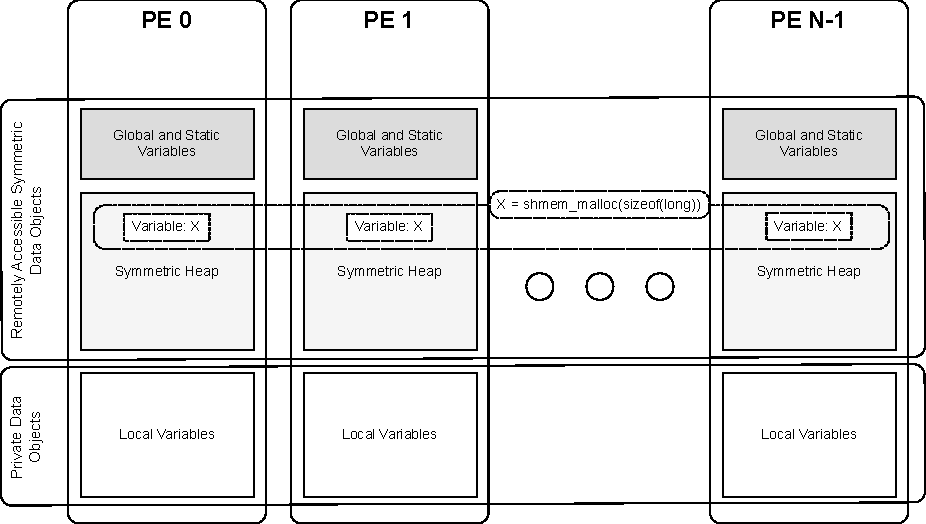
\includegraphics[width=\textwidth]{img/pgas-oshm-addressspace}
\caption{Visualization of the symmetric shared address space in \acs{OpenSHMEM}. Image adapted from \cite[ch.~3]{oshm-std}.}
\label{img:background:oshm:addressspace}
\end{figure}

The basic communication primitives in \ac{OpenSHMEM} are \code{sh\-mem\_put} and \code{sh\-mem\_get}, along with their non-blocking counterparts \cite[ch.~9.6]{oshm-std}. These routines simply copy data from one source buffer to a target \ac{PE}. The specification of a target buffer is not required due to the symmetric memory layout. Results of non-blocking function calls are guaranteed to be visible after a call to the function \code{shmem\_quiet} which blocks until the previously issued transfers have concluded \cite[ch.~9.11.2]{oshm-std}.

Apart from the simple transfer routines a selection of collective operations is available. Barriers come in two shapes: A global barrier synchronizes all \acp{PE}. Alternatively, \acp{PE} can be grouped into \emph{teams} which may be synchronized independently with the \code{shmem\_sync} function \cite[ch.~9.9.3]{oshm-std}. In contrast to the \code{shmem\_sync} routine, the traditional barrier function contains an implicit \code{shmem\_quiet} which waits for all outstanding transfers to complete. Further collective operations include \emph{broadcast}, \emph{reduce} and \emph{collect}. The collection operation concatenates several blocks of data in the shared memory into a consecutive block at every participating \ac{PE} \cite[ch.~9.9.8]{oshm-std}. For concurrently accessing objects in shared memory \ac{OpenSHMEM} also provides features of locks and atomic operations \cite[ch.~9.12.1, ch.~9.7]{oshm-std}.

An evaluation of the \ac{OpenSHMEM} reference implementation can be found in \cite{oshm-eval}. The provided application benchmarks implement the \ac{NPB} and evalute the performance against \ac{MPI}-1 and \ac{MPI}-2. The obtained results are not meant to show that \ac{OpenSHMEM} performs better than \ac{MPI}, since the implementation under test is mostly unoptimized, as the authors claim. It is, however, well illustrated that \ac{OpenSHMEM} is a functioning \ac{PGAS} implementation that can be integrated into distributed \ac{HPC} applications without a significant loss of performance.


\section{\acs{MPI}}

\Ac{MPI} is the current de facto standard for parallel communication \acp{API}. In \ac{MPI} a vast number of routines for point-to-point communication, one-sided communication, collective operations and synchronization is provided, making \ac{MPI} suitable for most applications \cite[ch.~3.3]{diss-end}.

In the traditional \ac{MPI}-1 standard, communication schemes are designed to be two-sided only. This means that in order to transfer data, the sender needs to call a sending routine such as \code{MPI\_Send} and the receiving process must call \eg \code{MPI\_Recv} in order to initiate the transfer. Consequently, both communication parties are involved in the transfer. There exist non-blocking versions of the sending and receiving routines to allow for asynchronous progress to the transfer operations without stalling the working processes for the full time that the transfer requires.

\begin{lstlisting}[style=cpp,captionpos={b},caption={Function definition of \code{MPI\_Irecv} {\cite[p.~51]{mpi3-std}}.},label=lst:background:mpi-irecv]
int MPI_Irecv(void *buf, int count, MPI_Datatype datatype, int source, int tag, MPI_Comm comm, MPI_Request *request);
\end{lstlisting}

An example of an asynchronous function definition is given in \autoref{lst:background:mpi-irecv}. In order to receive data, the receiving buffer is specified along with information on how much data is to be received. The \code{source} field specifies the rank from which the data originates. A rank is the same entity that \ac{OpenSHMEM} considers to be a \ac{PE} or which \ac{UPC} calls a thread. In contrast to the routines discussed before in \ac{OpenSHMEM} or \ac{UPC}, transactions can be marked by using the \code{tag} field. By this means, different types of communication can be differentiated if \eg multiple threads in the same process are involved in the communication and the order of posted sends do no longer define the order of the expected data at the receiving end. The \code{comm} field provides support for different \emph{communicators}. A communicator is conceptually equivalent to a team in \ac{OpenSHMEM}: A number of ranks can be aggregated under a communicator so that operations such as barriers are only applied to a specific selection of ranks that are involved in a certain processing scheme. The last parameter \code{request} is an output parameter that provides status information on the asynchronous progress of the function. Since \code{MPI\_Irecv} returns immediately without guaranteeing that the transfer is complete, means to check for the progress of the transfer must be implemented. This is done with the \code{MPI\_Wait} or \code{MPI\_Test} functions that interpret the \code{request} object generated by \code{MPI\_Irecv} and either wait until the operation has concluded or return immediately and provide information if the operation is finished yet or not.

This two-sided message passing scheme allows for a comprehensible usage in most applications. Due to the involvement of all ranks in the communication procedure, different program code needs to be managed for every rank. This is often error-prone when modifying algorithms, since the code of all ranks must be changed in the correct way. To alleviate this issue, one-sided communication provides an alternative way that has already been presented in \secref{sec:background:openshmem}. One-sided communication was introduced to \ac{MPI} with the \ac{MPI}-2 release of the specification and further expanded with \ac{MPI}-3 \cite[p.~iii]{mpi3-std}. The concepts how one-sided communication is used are, however, very different from \ac{OpenSHMEM}.

One-sided communication is preferably implemented using \ac{RMA}. If adequate interconnection hardware such as Infiniband is supplied, \ac{RMA} operations can be mapped to distinct hardware \cite[ch.~3.2]{upc-infiniband}. Otherwise, the transfer must be administered by the \ac{CPU} which affects the achievable communication performance adversely. In \ac{MPI} there are two options how \ac{RMA} operations can be initiated: 
\begin{itemize}
	\item Active target communication
	\item Passive target communication
\end{itemize}
With active target communication, both communication parties are involved in the transaction like in two-sided communication. In contrast to the previously presented scheme, one party is only involved in synchronization, whereas the other party performs the transfer when using active target communication. Passive target communication is closer to true one-sided communication because no program code is necessary on the remote rank to process the data transaction \cite[ch.~11.5]{mpi3-std}. Even if active target communication may seem counter-intuitive for a one-sided scheme, it has useful applications: In a parallel program, certain buffer locations may not be overwritten or read by a remote process at arbitrary times. With active target communication, a window in the program's flow may be specified when remote access is sensible in the application's context. Using passive target communication it must be ensured by other means that the remote data is either valid or not actively used to allow for memory consistency.

Active target communication specifies the access period with the term \emph{epoch}. An \ac{RMA} epoch can be initiated and terminated; all \ac{RMA} calls must be issued between the initiation and termination call of the epoch \cite[p.~437]{mpi3-std}. Synchronization always happens with respect to a certain memory window which has to be created on all ranks prior to any \ac{RMA} function calls. The simplest form of active target communication is realized via the \code{MPI\_Fence} operation which forces all previously issued \ac{RMA} operations to conclude \cite[p.~440\,f]{mpi3-std}. The call starts and end \ac{RMA} epochs -- therefore any \ac{RMA} transactions must be wrapped in \code{MPI\_Fence} function calls. Because the fence operation forces synchronization on the entire memory window which can be costly, a more flexible approach may be used instead. With \ac{PSCW} synchronization, the start and end of an epoch may be defined specifically on each participating rank: The initiator of the transfer calls the \enquote{start} function, issues all its \ac{RMA} calls and then concludes the epoch with the \enquote{complete} function. The remote end calls the \enquote{post} function whenever it is able to accept incoming \ac{RMA} transactions. It terminates the exposure of the memory window by calling the \enquote{wait} function after which all \ac{RMA} operations have been completed at the remote end. A visualization of the scheme is depicted in \autoref{img:background:mpi:pscw}. This avoids possible data races and provides maximum flexibility \cite[ch.~11.5.2]{mpi3-std}. Unfortunately, this more complex scheme requires more program logic and is therefore more difficult to maintain.

\begin{figure}[htb]
\centering
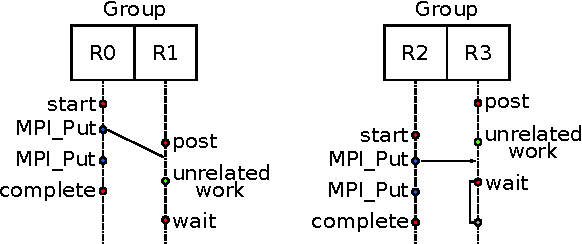
\includegraphics[width=0.8\textwidth]{img/mpi-pscw}
\caption{Visualization of the \ac{PSCW} scheme. Adopted from \cite{mpi-pscw-img}.}
\label{img:background:mpi:pscw}
\end{figure}

Passive target communication delegates the synchronization of allowing memory accesses to the user. To transfer data using passive target communication only a lock has to be obtained for the window which has to be released after all \ac{RMA} operations are issued \cite[ch.~11.5.3]{mpi3-std}. The necessity for locks stem from the parallel nature of the program: While consecutive memory read operations do not impose issues, multiple writes  from different ranks to the same window may lead to memory consistency issues \cite[ch.~8.4]{mpi-pscw-img}. The release of the lock does not imply that operations are concluded -- a subsequent flush operation is required to ensure that buffers may be reused \cite[ch.~11.5.4]{mpi3-std}.

Apart from functions and concepts to send and receive raw data, numerous collective operations are defined. Examples encompass \emph{scatter}, \emph{gather}, \emph{broadcast}, \emph{reduce} and \emph{barrier}. All of the functions mentioned exist in different forms to differentiate between blocking behavior and to control if possible results are pushed to all ranks \cite[ch.~5]{mpi3-std}.

Since \ac{MPI} is the de facto standard of distributed communication, it is widely adopted and multiple implementations of the \ac{API} exist for various application fields. Although \ac{MPI} is not a real \ac{PGAS} language, it has incorporated \ac{PGAS} features through the extension of memory windows and one-sided communication.

\section{\acs{GASPI}}

With \ac{GASPI} the last \ac{PGAS} approach will be introduced in this work. \Ac{GASPI} is mostly comparable to \ac{OpenSHMEM} as it incorporates explicit remote read or write routines and does not support true global address space access like \ac{UPC} \cite[p.~31\,f.]{gaspi-sum}. In contrast to \ac{OpenSHMEM}, \ac{GASPI} supports the segmentation of the memory in multiple parts. A possible segmentation of the global address space is shown in \autoref{img:background:gaspi:addressspace}. These \emph{memory segments} may be defined differently on every node, thus \ac{GASPI} does not enforce a symmetric memory model \cite[p.~19]{gaspi-sum}. Consequently, a specific memory location is defined by the triple of the remote rank, the segment identifier and a byte offset inside the remote segment \cite[p.~23]{gaspi-sum}.

\begin{figure}[htb]
\centering
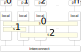
\includegraphics[width=0.8\textwidth]{img/pgas-gaspi-addressspace}
\caption{Visualization of the segmented global address space in \acs{GASPI}. Image adapted from \cite[ch.~3.5.1]{diss-end}.}
\label{img:background:gaspi:addressspace}
\end{figure}


The fundamental functions used for data exchange are \code{gas\-pi\_read} and \code{gas\-pi\_write} \cite[ch.~8.2]{gaspi-std}. Their function definitions are depicted in \autoref{lst:background:gaspi-write} and \autoref{lst:background:gaspi-read}. Apart from the triple for addressing memory locations at the local and the remote site, a queue and a timeout need to be specified. 

\begin{lstlisting}[style=cpp,captionpos={b},caption={Function definition of \code{gaspi\_write} {\cite[ch.~8.2.1]{gaspi-std}}.},label=lst:background:gaspi-write]
gaspi_return_t gaspi_write ( 
	gaspi_segment_id_t segment_id_local,
	gaspi_offset_t offset_local,
	gaspi_rank_t rank,
	gaspi_segment_id_t segment_id_remote,
	gaspi_offset_t offset_remote,
	gaspi_size_t size,
	gaspi_queue_id_t queue,
	gaspi_timeout_t timeout
)
\end{lstlisting}

\begin{lstlisting}[style=cpp,captionpos={b},caption={Function definition of \code{gaspi\_read} {\cite[ch.~8.2.2]{gaspi-std}}.},label=lst:background:gaspi-read]
gaspi_return_t gaspi_read ( 
	gaspi_segment_id_t segment_id_local,
	gaspi_offset_t offset_local,
	gaspi_rank_t rank,
	gaspi_segment_id_t segment_id_remote,
	gaspi_offset_t offset_remote,
	gaspi_size_t size,
	gaspi_queue_id_t queue,
	gaspi_timeout_t timeout 
)
\end{lstlisting}

\subsection{Queues}

Queues are a new concept in \ac{GASPI}; the already presented other \ac{PGAS} approaches do not feature the notion of different queues. In \ac{GASPI}, communication operations need to be posted to a specific queue. Queues can either be created dynamically at runtime up to a certain maximum amount or a set of queues can be used that is available by default. There are getter functions to determine which queue identifiers represent valid queues \cite[ch.~6.5.1]{gaspi-std}. Only weak ordering guarantees are made for operations that are posted to a queue: Essentially, most operations may be processed in any given order. The important exception concerns notifications which exist as synchronization primitives. If data transferring operations such as \code{gaspi\_read} or \code{gaspi\_write} are succeeded by a notification to the same rank in the same queue as the transfer operation, it is guaranteed that the operation and all prior operations to the same rank and the same queue are completed and processed in order when the notification is received \cite[ch.~8.3.2]{gaspi-std}.

Queues have a fixed size that is implementation-specific. If a submission to the desired queue fails due to a queue overrun, the return value of \code{gaspi\_read} or \code{gaspi\_write} will provide this information. When developing \ac{GASPI} applications it is desirable to keep track of the return values provided by the \ac{GASPI} functions to detect possible failures. All \ac{GASPI} functions return a value of the type \code{gaspi\_return\_t} which is an enumeration type over all possible error situations. If a queue is full, submissions may either be posted to a different queue or the application may wait by using \code{gas\-pi\_wait}  until the queue is empty again. The implementation of the \ac{GASPI} standard ensures that all queues are treated in a fair fashion and that queue entries do not remain in the queue for an indefinite amount of time \cite[ch.~8.1]{gaspi-std}.

\subsection{Timeouts}

The last parameter in \autoref{lst:background:gaspi-write} and \autoref{lst:background:gaspi-read} is \code{timeout} which corresponds to another special feature of \ac{GASPI}. All remote operations feature a timeout that may be either specified in milliseconds or as a special value \cite[ch.~3.9]{gaspi-std}. Special values are \code{GASPI\_BLOCK} and \code{GASPI\_TEST}. The first value causes the function to wait as long as it takes for the respective operation to complete. \code{GASPI\_TEST} lets the respective function return as soon as possible. Note that  \code{gaspi\_read} or \code{gaspi\_write} returns if the \ac{RMA} request as been successfully submitted to the queue which will subsequently be processed in an asynchronous fashion. Providing the \code{GASPI\_BLOCK} value for both functions only means that writing the request in the queue will be done in a blocking fashion; the \ac{RMA} transaction itself will be handled by the library without blocking behavior in the application \cite[p.~60\,f.]{gaspi-std}.

\subsection{Synchronization Primitives}

In comparison to \ac{MPI}, \ac{GASPI} uses a different concept for synchronization: The only technique to ensure that an \ac{RMA} access has been completed is by exchanging notifications. A barrier call combined with a wait statement is not sufficient, since the wait functions only ensure that local operations have been completed \cite[p.~20]{gaspi-tut}. To send a notification, the function \code{gaspi\_notify} may be used \cite[ch.~8.3.2]{gaspi-std}. Its formal definition is shown in \autoref{lst:background:gaspi-notify}.

\begin{lstlisting}[style=cpp,captionpos={b},caption={Function definition of \code{gaspi\_notify} {\cite[ch.~8.3.2]{gaspi-std}}.},label=lst:background:gaspi-notify]
gaspi_return_t gaspi_notify ( 
	gaspi_segment_id_t segment_id,
	gaspi_rank_t rank,
	gaspi_notification_id_t notification_id,
	gaspi_notification_t notification_value,
	gaspi_queue_id_t queue,
	gaspi_timeout_t timeout 
)
\end{lstlisting}

As it is visible from \autoref{lst:background:gaspi-notify}, notifications are bound to a memory segment, a target rank and a queue. Furthermore, notifications may be tagged by using an identifier. This is useful, if \eg multiple write operations are issued to the same target from multiple ranks in parallel. Without tagging the notifications, race conditions occur that causes notifications to be overwritten. Similar to the read or write operations, issuing a notification requires a slot in the given queue. To avoid the potential loss of notifications it needs to be checked that the notification has been successfully posted to the queue. Additionally, a notification value may be provided for transporting user-specific status codes.

\subsection{Advanced \acs{RMA} Functions}

Initiating an \ac{RMA} operation followed by a subsequent notification is a typical scenario in algorithms. Therefore, special functions exist that send a notification directly after the \ac{RMA} operation. The functions \gaspiWriteNotify and \gaspiReadNotify implement this behavior. Consequently, calling these functions requires at least two empty slots in the given queue: One for the \ac{RMA} operation and one for the notification \cite[ch.~8.4]{gaspi-std}. The target rank that receives the notification differs when calling  \gaspiWriteNotify or \gaspiReadNotify. With \gaspiWriteNotify, the \ac{RMA} operation targets a specific remote rank and deploys its data there; the subsequent notification is sent to the same rank to inform the remote rank that the data is now available \cite[ch.~8.4.1]{gaspi-std}. When \gaspiReadNotify is used, the notification is sent to the rank that receives the data -- the remote rank from where the data is fetched is not involved in the operation in any way \cite[ch.~8.4.4]{gaspi-std}.

\subsection{Collective and Atomic Operations}
\label{ssec:background:gaspi:collective-atomic}

Apart from the basic messaging functions, a small selection of collective and atomic operations are defined. Most prominent is the barrier function \code{gaspi\_barrier} which is given a group identifier and a timeout. Groups are an equivalent concept as teams in \ac{OpenSHMEM} and allow the creation of subsets of ranks which may operate on different independent problems. A barrier does therefore not need to be global across all ranks but may be issued in a more specific way \cite[ch.~11.2.1]{gaspi-std}. Besides the barrier, the only other collective operation defined in the \ac{GASPI} standard is the allreduce operation. The procedure combines an array of elements on each rank involved element-wise under a given operator and distributes the result to every node. 

\begin{lstlisting}[style=cpp,captionpos={b},caption={Function definition of \code{gaspi\_allreduce} {\cite[ch.~11.3.1]{gaspi-std}}.},label=lst:background:gaspi-allreduce]
gaspi_return_t gaspi_allreduce ( 
	gaspi_const_pointer_t buffer_send,
	gaspi_pointer_t buffer_receive,
	gaspi_number_t num,
	gaspi_operation_t operation,
	gaspi_datatype_t datatype,
	gaspi_group_t group,
	gaspi_timeout_t timeout
)
\end{lstlisting}

When inspecting the function definition in \autoref{lst:background:gaspi-allreduce} the most obvious difference to the aforementioned data-transferring routines is that local memory buffers are used instead of a memory specification inside a global memory segment. Copying the data into a globally visible buffer is done internally by the routine itself \cite[ch.~11.3.1]{gaspi-std}. Another fact worth mentioning is the function's behavior when the timeout is exceeded either by providing \code{GASPI\_TEST} to the function or if the number of milliseconds given has run out. The function keeps an internal state that allows the continuation after another call to the routine. This can be used to hide the \ac{RMA} latency by performing other unrelated work. The allreduce operation is available with three predefined element operations for calculating the minimum, the maximum and the sum of the given distributed array. With an alternative function, a custom element-processing routine may be specified that allows the implementation of arbitrary allreduce operations.

Next to the collective operations, two atomic functions are defined: \emph{compare and swap} and \emph{fetch and add} \cite[ch.~10]{gaspi-std}. Their primary benefit is to provide means of synchronizing access to shared datastructures on globally visible memory segments. Another way of using atomic counters is for dynamic load distribution schemes, as pointed out in \cite[ch.~6]{gaspi-sum}.

\subsection{Two-Sided Communication}
\label{ssec:background:gaspi:two-sided}

Apart from the previously discussed routines for one-sided communication, the \ac{GASPI} standard also supports  \enquote{traditional} two-sided communication. Conceptually, these routines are similar to the \ac{MPI}-1 communication functions but they differ from the known two-sided schemes in some ways: First, the target memory destination or source needs to be specified as part of the global address space. Therefore, memory needs to be given as segment identifier, target rank and byte offset. Second, all two-sided operations are handled via special internal queues whose capacity is not visible to the user \cite[ch.~9.2]{gaspi-std}. Furthermore, the amount of data transferable with the two-sided communication routines is heavily limited. The implementation-specific limit can be investigated by querying the function \code{gaspi\_\allowbreak passive\_\allowbreak transfer\_\allowbreak size\_\allowbreak max} \cite[ch.~12.4.1]{gaspi-std}.

The main purpose for two-sided communication is data exchange where the rank of the data source is unknown from the perspective of the receiver or if there is need for synchronization directly after a transfer \cite[ch.~9.1]{gaspi-std}. The two-sided communication routines \gaspiPassiveSend and \gaspiPassiveReceive therefore provide a simpler interface to accomplish this in comparison to issuing a \ac{RMA} put operation followed by a queue flush and a matching wait on a notification on the remote end. The part \emph{passive} in the function name is meant to indicate that the two functions may block without using busy waiting. This means that waiting on a function call should not consume \ac{CPU} cycles in the application \cite[ch.~9.1]{gaspi-std}.

\subsection{Fault Tolerance}
\label{ssec:background:gaspi:fault-tolerance}
The final feature of \ac{GASPI} that is regarded as special is fault tolerance \cite[ch.~8.2]{gaspi-sum}. In large scale \ac{HPC} systems node failures or networking faults may occur at arbitrary times. When the possibility of faults is not addressed when designing the application, the program will either stall indefinitely or crash, causing the progress made so far to be lost. In \ac{GASPI}, means of detecting failures in the system is provided: The application may choose to inspect the \ac{GASPI} state vector \cite[ch.~5.5]{gaspi-std}. In case of a failure in the progress of a communication operation, the state vector may read \code{GASPI\_STATE\_CORRUPT} for a specific rank. This allows the application to perform a graceful application shutdown in the least; optimally a hot-standby node may be started by the runtime environment which can subsequently be integrated in the running computation. The \ac{GASPI} standard, however, does not demand this advanced feature to be implemented. To make use of the fault tolerance features of \ac{GASPI}, applications must use the timeout value demanded by every non-local \ac{GASPI} function. If \code{GASPI\_BLOCK} is supplied with function calls, the operation stalls for an infinite amount of time in case a fault occurs; this special timeout value must therefore be avoided when writing fault-tolerant programs \cite[ch.~3.9]{gaspi-std}. At the time of writing, the open source reference implementation of the \ac{GASPI} standard \acs{GPI}-2 does not support dynamic node insertion required for fault tolerance \cite{gpi-2-github}.